\chapter{RESULTS}
\label{ch:results}

\section{Introduction}

This chapter presents comprehensive results from training and evaluating three state-of-the-art deep learning architectures on slice-level brain tumor detection. We compare EfficientNet-B2, ResNet-50, and DeiT-Base across quantitative performance metrics and qualitative explainability analysis using Grad-CAM visualizations.

\section{Dataset Statistics}

\subsection{BraTS 2021 Task 1 - Patient-Level Splitting}

The dataset comprises 1,251 glioblastoma patients from BraTS 2021, split at the patient level to ensure reliable generalization estimates:

\begin{table}[h]
\centering
\caption{Dataset distribution with patient-centric splitting (code-only, seed=42)}
\label{tab:dataset_stats}
\begin{tabular}{lcc}
\toprule
\textbf{Split} & \textbf{Patients} & \textbf{Approx. Slices} \\
\midrule
Training & 877 & $\sim$136,000 \\
Validation & 187 & $\sim$29,000 \\
Test & 187 & $\sim$29,000 \\
\midrule
\textbf{Total} & \textbf{1,251} & $\sim$\textbf{194,000} \\
\bottomrule
\end{tabular}
\end{table}

\noindent Each patient contributes approximately 155 axial slices, resulting in a large-scale slice-level classification dataset. Ground truth labels are derived from expert-annotated tumor segmentation masks: slices with any tumor pixels (segmentation $>$ 0) are labeled positive (1), otherwise negative (0).

\textbf{Class distribution characteristics:}
\begin{itemize}
    \item Majority of slices are tumor-free (only $\sim$40\% of brain volume contains tumor)
    \item Natural class imbalance requires F1-score evaluation alongside accuracy
    \item Patient-centric batching ensures all slices from one patient processed together
\end{itemize}

\section{Training Progression and Convergence}

All models were trained for 10 epochs using two-stage transfer learning: backbone frozen (epochs 0-4), then full fine-tuning (epochs 5-9). Training converged rapidly due to large dataset size and effective pretrained features. Figure \ref{fig:training_curves} shows the training and validation curves for all three models.

\begin{figure}[H]
\centering
\begin{subfigure}[b]{\textwidth}
    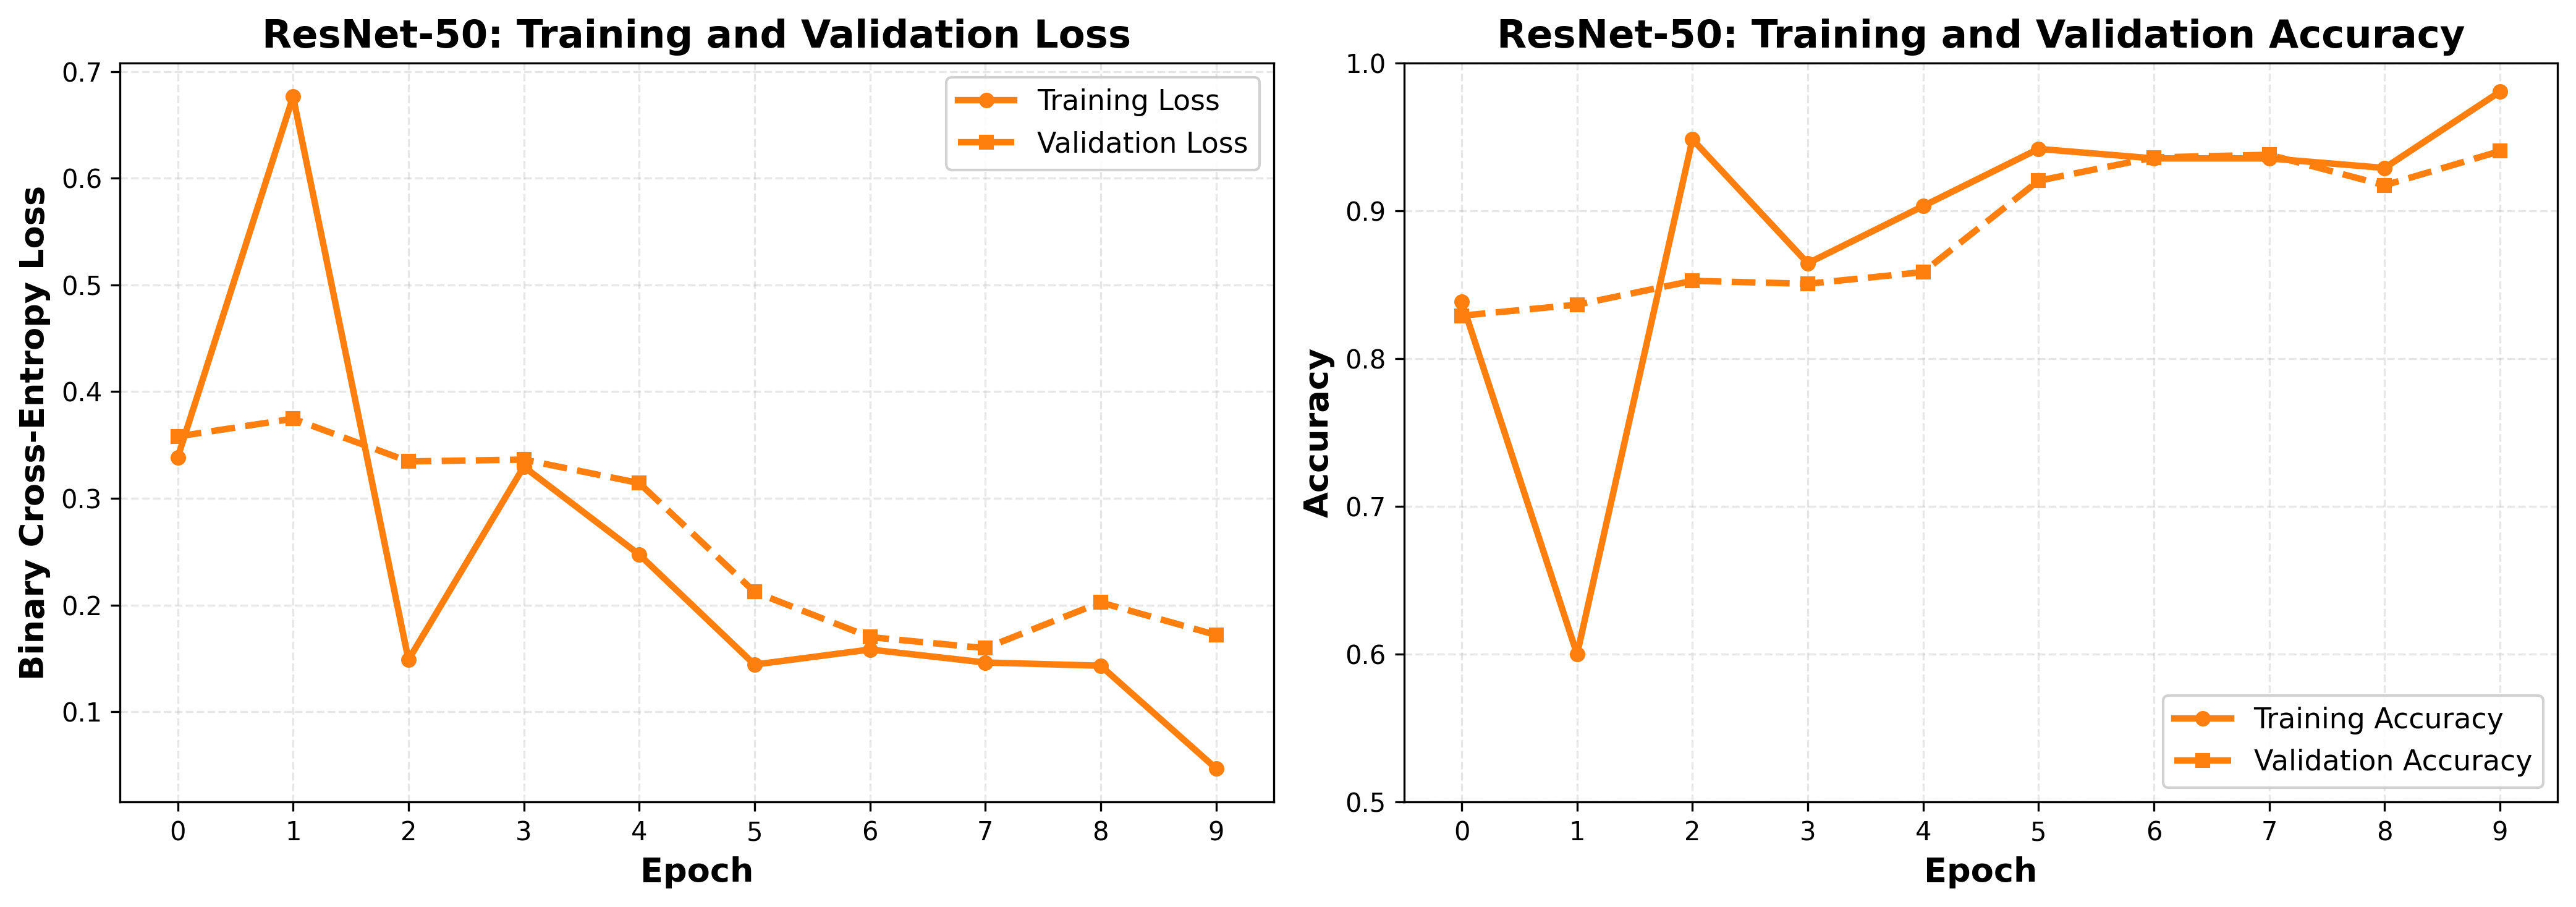
\includegraphics[width=\textwidth]{figures/training_curves_resnet_50.png}
    \caption{ResNet-50 training curves}
\end{subfigure}
\vspace{0.3cm}
\begin{subfigure}[b]{\textwidth}
    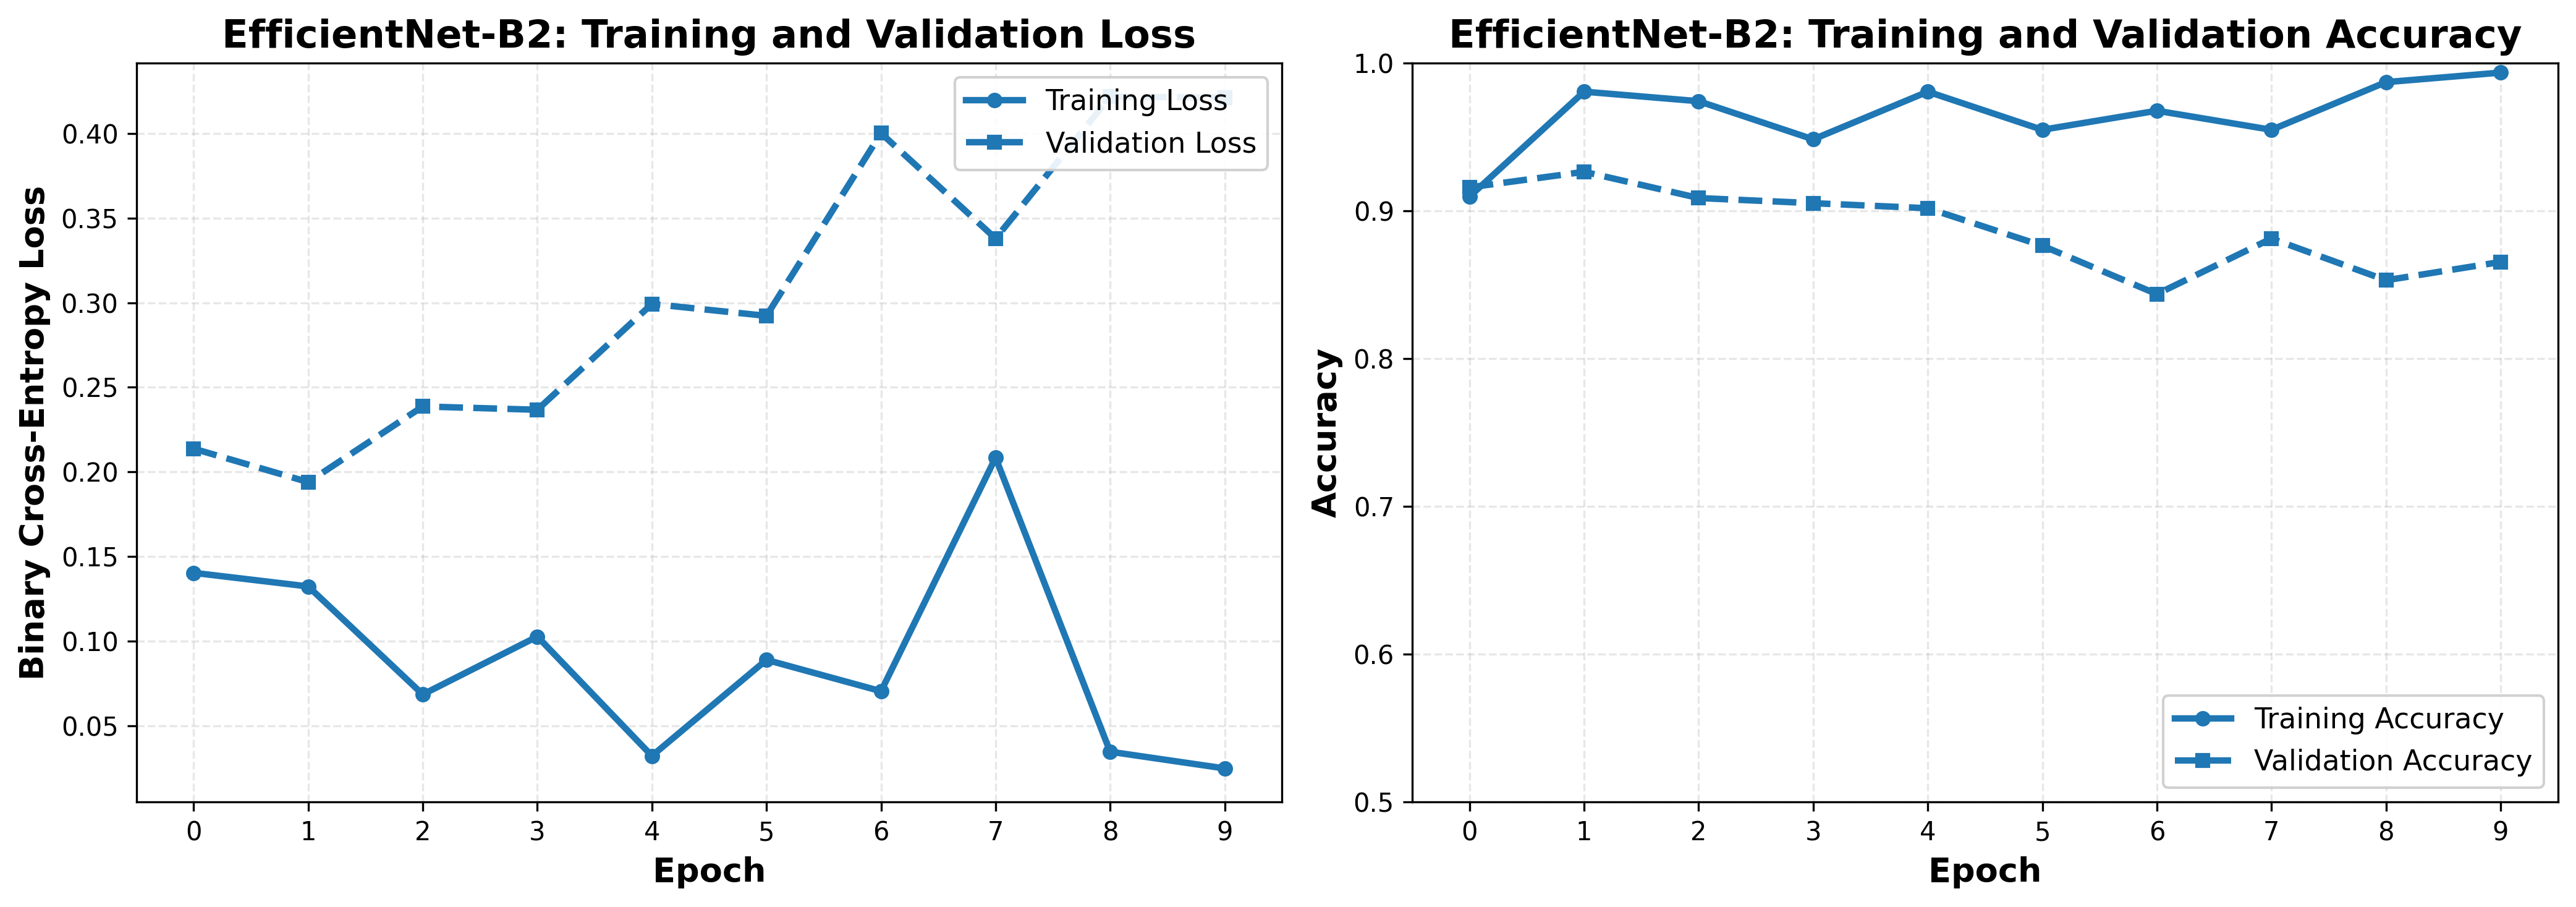
\includegraphics[width=\textwidth]{figures/training_curves_efficientnet_b2.png}
    \caption{EfficientNet-B2 training curves}
\end{subfigure}
\vspace{0.3cm}
\begin{subfigure}[b]{\textwidth}
    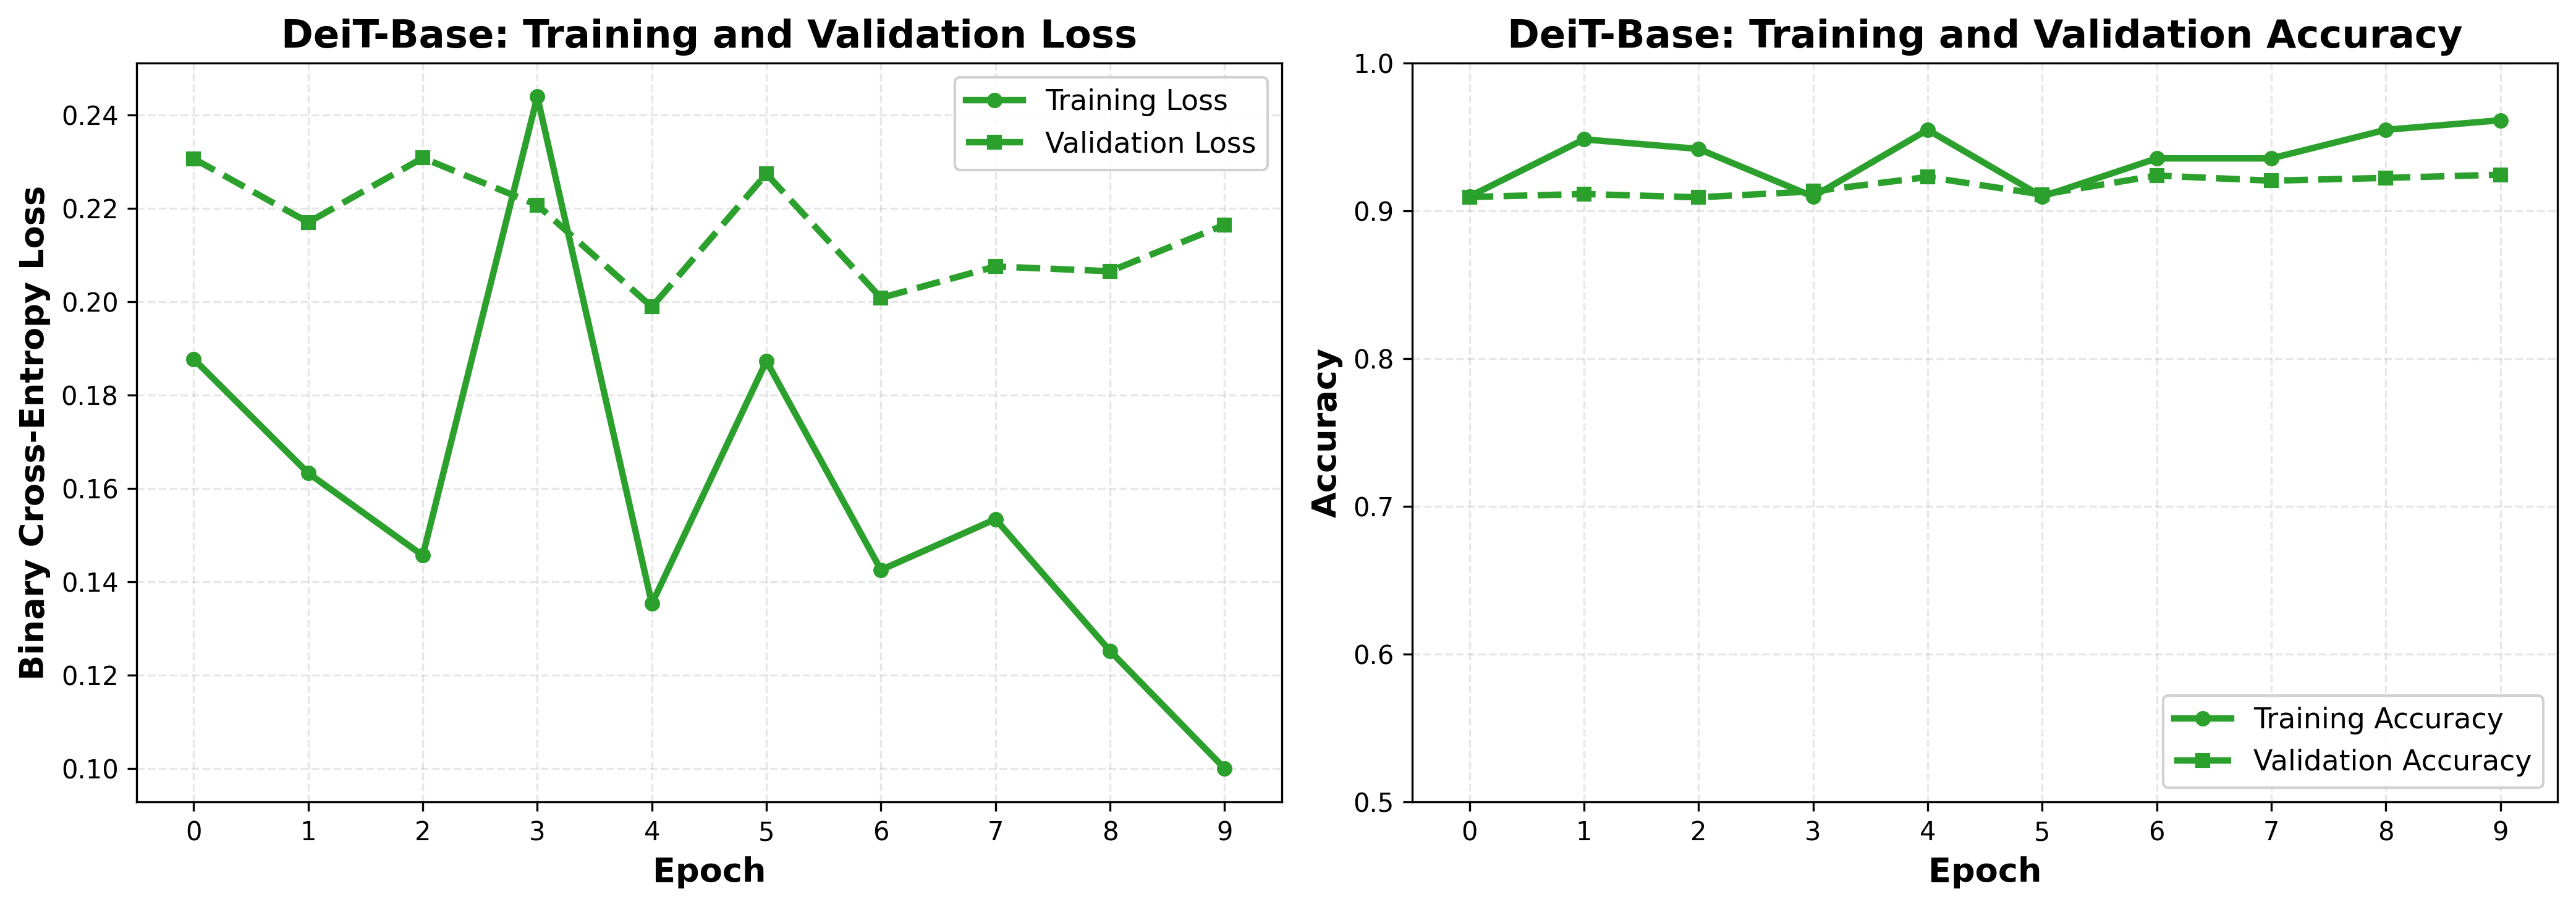
\includegraphics[width=\textwidth]{figures/training_curves_deit_base.png}
    \caption{DeiT-Base training curves}
\end{subfigure}
\caption{Training and validation curves showing loss and accuracy progression over 10 epochs for all three models. Note the rapid convergence and stable training dynamics.}
\label{fig:training_curves}
\end{figure}

\subsection{Convergence Behavior}

\begin{itemize}
    \item \textbf{EfficientNet-B2}: Achieved best validation accuracy at epoch 1 (92.64\%), showing immediate strong transfer from ImageNet features
    \item \textbf{ResNet-50}: Converged at epoch 9 (94.04\% validation accuracy) after full backbone fine-tuning
    \item \textbf{DeiT-Base}: Achieved best validation at epoch 9 (92.44\%), demonstrating slower but stable convergence typical of transformers
\end{itemize}

The rapid convergence of EfficientNet-B2 suggests its compound-scaled architecture provides highly transferable features for medical imaging, while ResNet-50's later convergence indicates benefit from prolonged fine-tuning of deeper residual connections.

\section{Test Set Performance}

Using checkpoints with best validation accuracy, we evaluate all three models on the held-out test set (187 patients, $\sim$29,000 slices). Results are summarized in Table \ref{tab:test_performance}.

\subsection{Quantitative Metrics}

\begin{table}[h]
\centering
\caption{Test set performance comparison on slice-level tumor detection}
\label{tab:test_performance}
\begin{tabular}{lccc}
\toprule
\textbf{Model} & \textbf{Test Accuracy} & \textbf{Test F1-Score} & \textbf{Test Loss} \\
\midrule
\textbf{ResNet-50} & \textbf{94.69\%} & \textbf{93.72\%} & \textbf{0.1495} \\
EfficientNet-B2 & 93.67\% & 92.70\% & 0.1650 \\
DeiT-Base & 93.46\% & 92.35\% & 0.1933 \\
\bottomrule
\end{tabular}
\end{table}

\textbf{Key findings:}

\begin{itemize}
    \item \textbf{ResNet-50 achieves best overall performance} (94.69\% accuracy, 93.72\% F1), demonstrating that deep residual CNNs remain highly effective for medical imaging when properly trained
    \item \textbf{EfficientNet-B2 ranks second} (93.67\% accuracy) despite having 3× fewer parameters than ResNet-50, showcasing parameter efficiency through compound scaling
    \item \textbf{DeiT-Base performs comparably} (93.46\% accuracy) despite being a pure transformer without CNN inductive biases, validating transformers for medical imaging
    \item \textbf{F1-scores closely match accuracy} across all models, indicating balanced performance on both positive and negative classes despite natural class imbalance
\end{itemize}

All three models achieve strong generalization ($>$93\% test accuracy), suggesting that:
\begin{enumerate}
    \item The 3-channel standard RGB approach (T1ce, T2, FLAIR) provides sufficient information for slice-level tumor detection
    \rev{\item ImageNet pretrained features transfer effectively to brain MRI}
    \item Patient-level splitting successfully prevents data leakage and pseudo-replication bias
\end{enumerate}

\subsection{Confusion Matrix Analysis}

Figure \ref{fig:confusion_matrices} presents slice-level confusion matrices for all three models, showing classification patterns on the test set.

\begin{figure}[H]
\centering
\begin{subfigure}[b]{0.48\textwidth}
    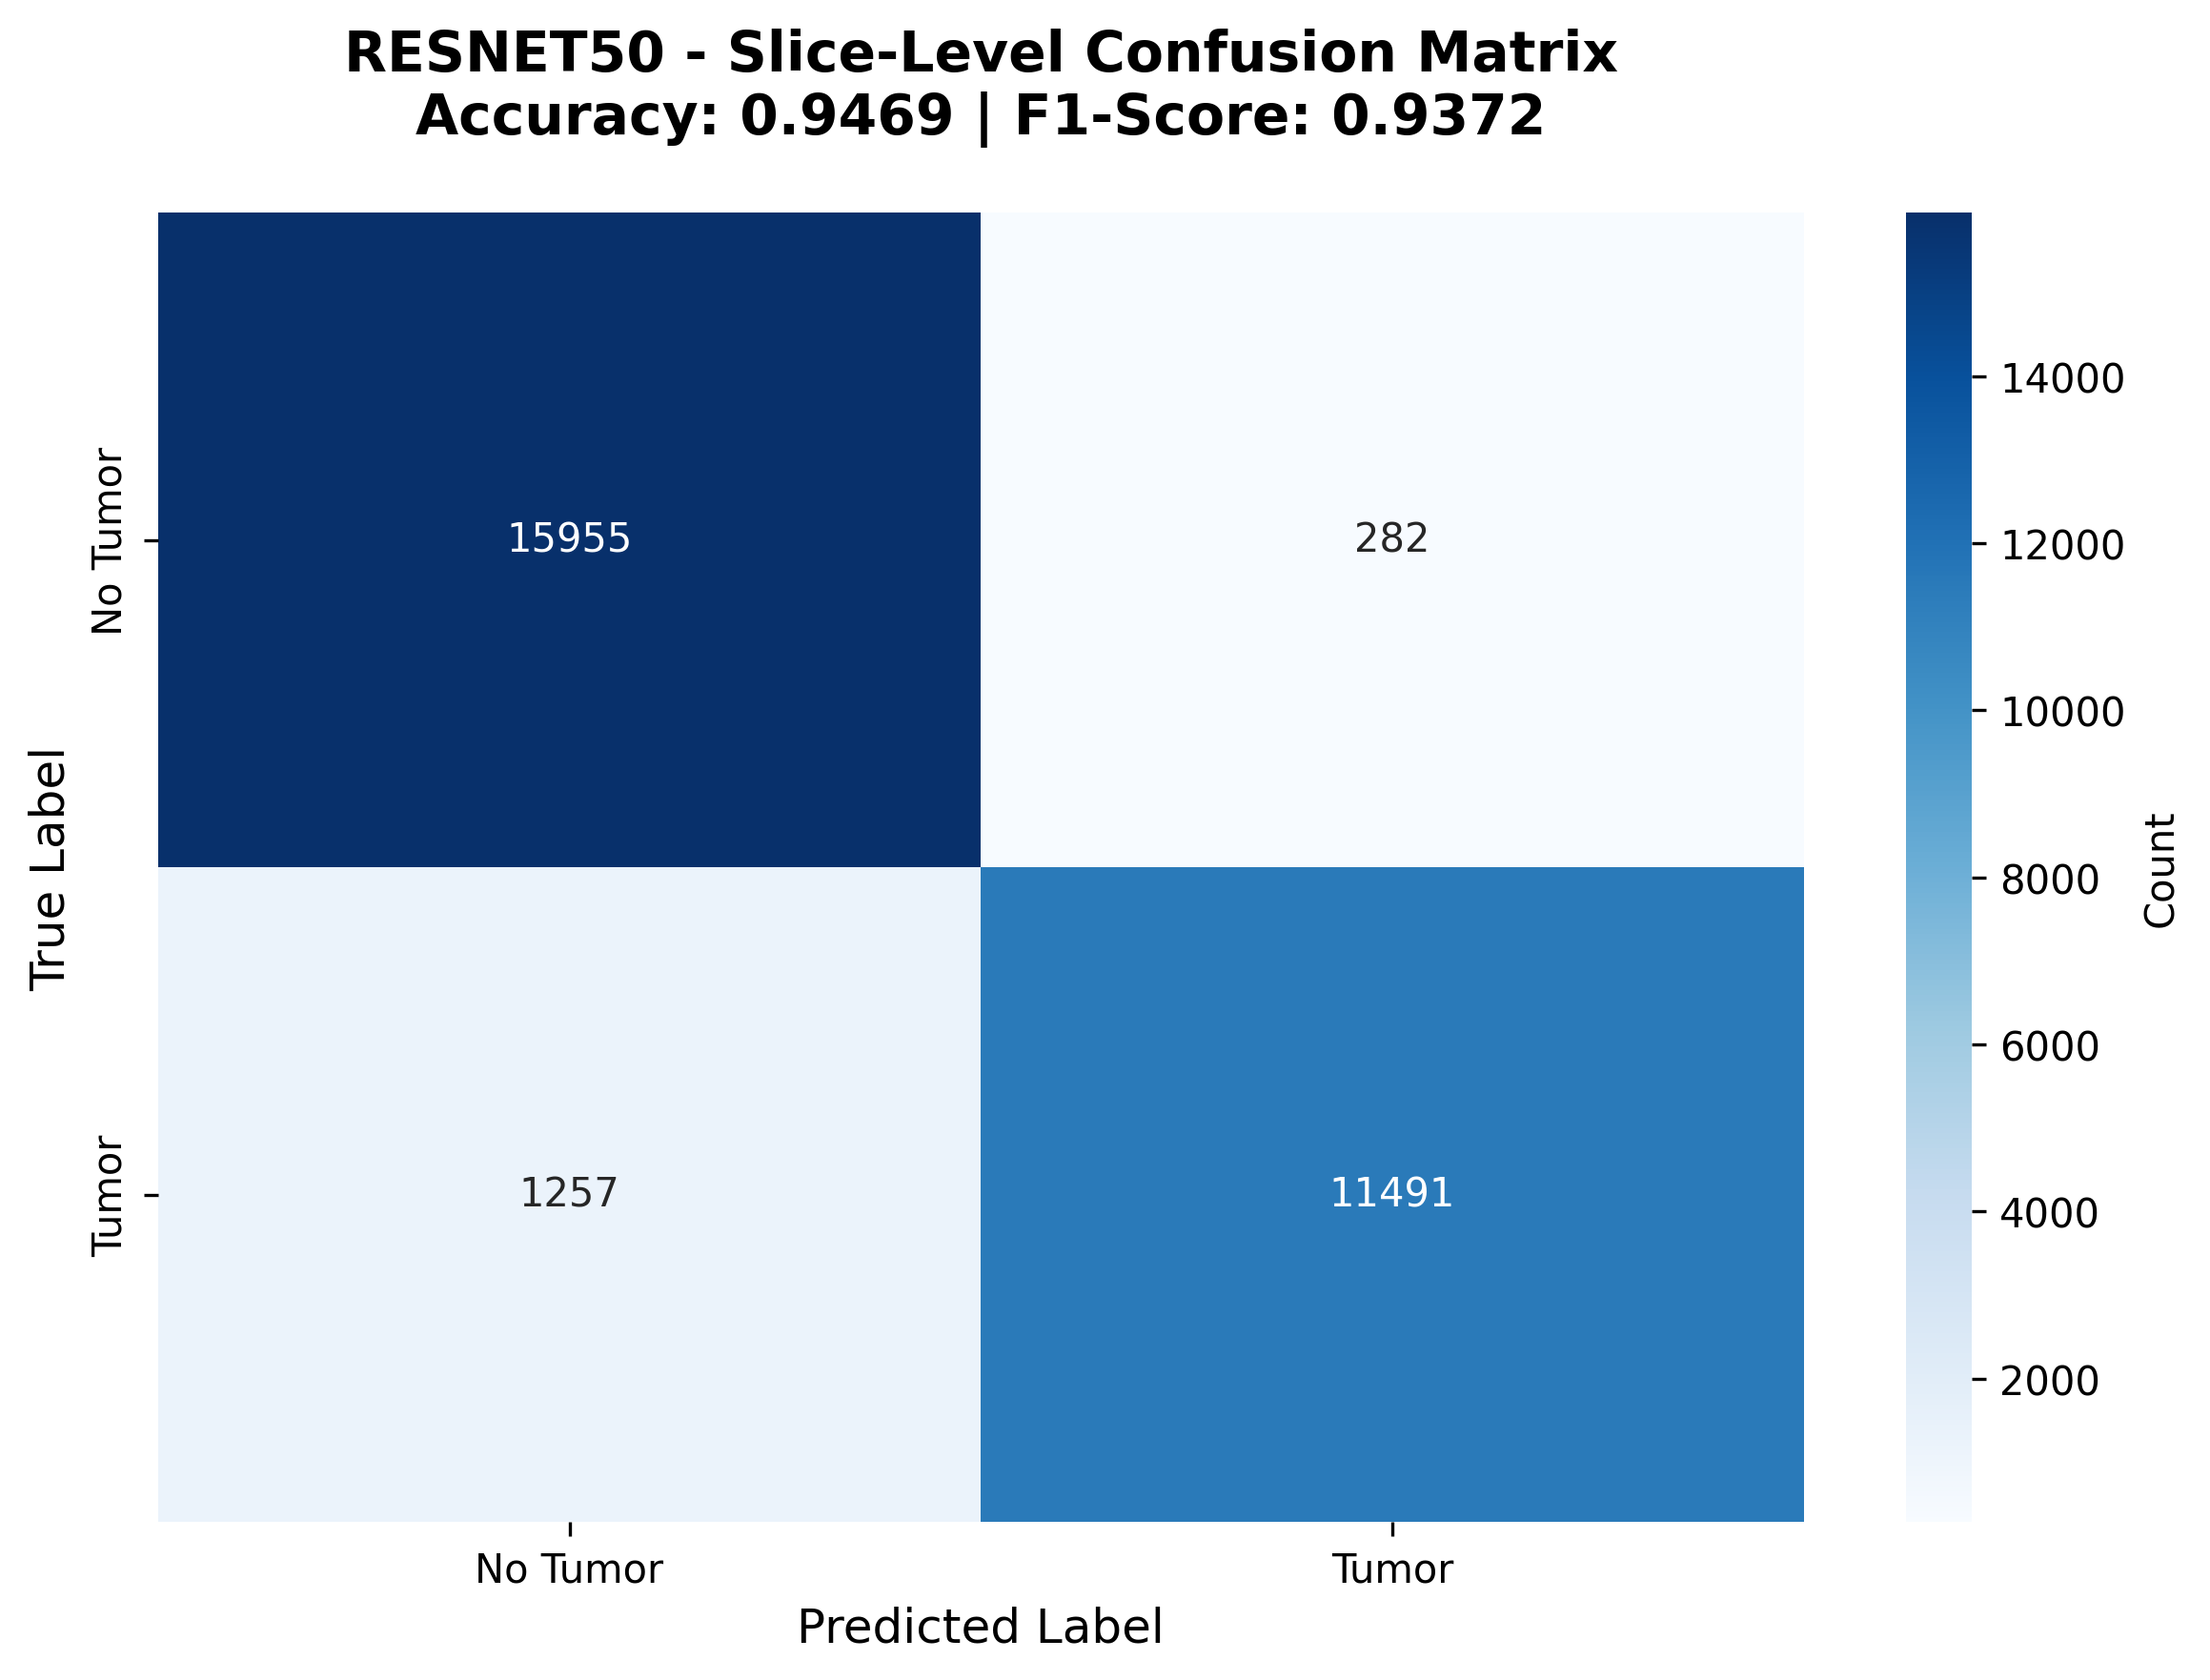
\includegraphics[width=\textwidth]{figures/cm_resnet50.png}
    \caption{ResNet-50: Best performance (94.69\% accuracy, 93.72\% F1)}
\end{subfigure}
\hfill
\begin{subfigure}[b]{0.48\textwidth}
    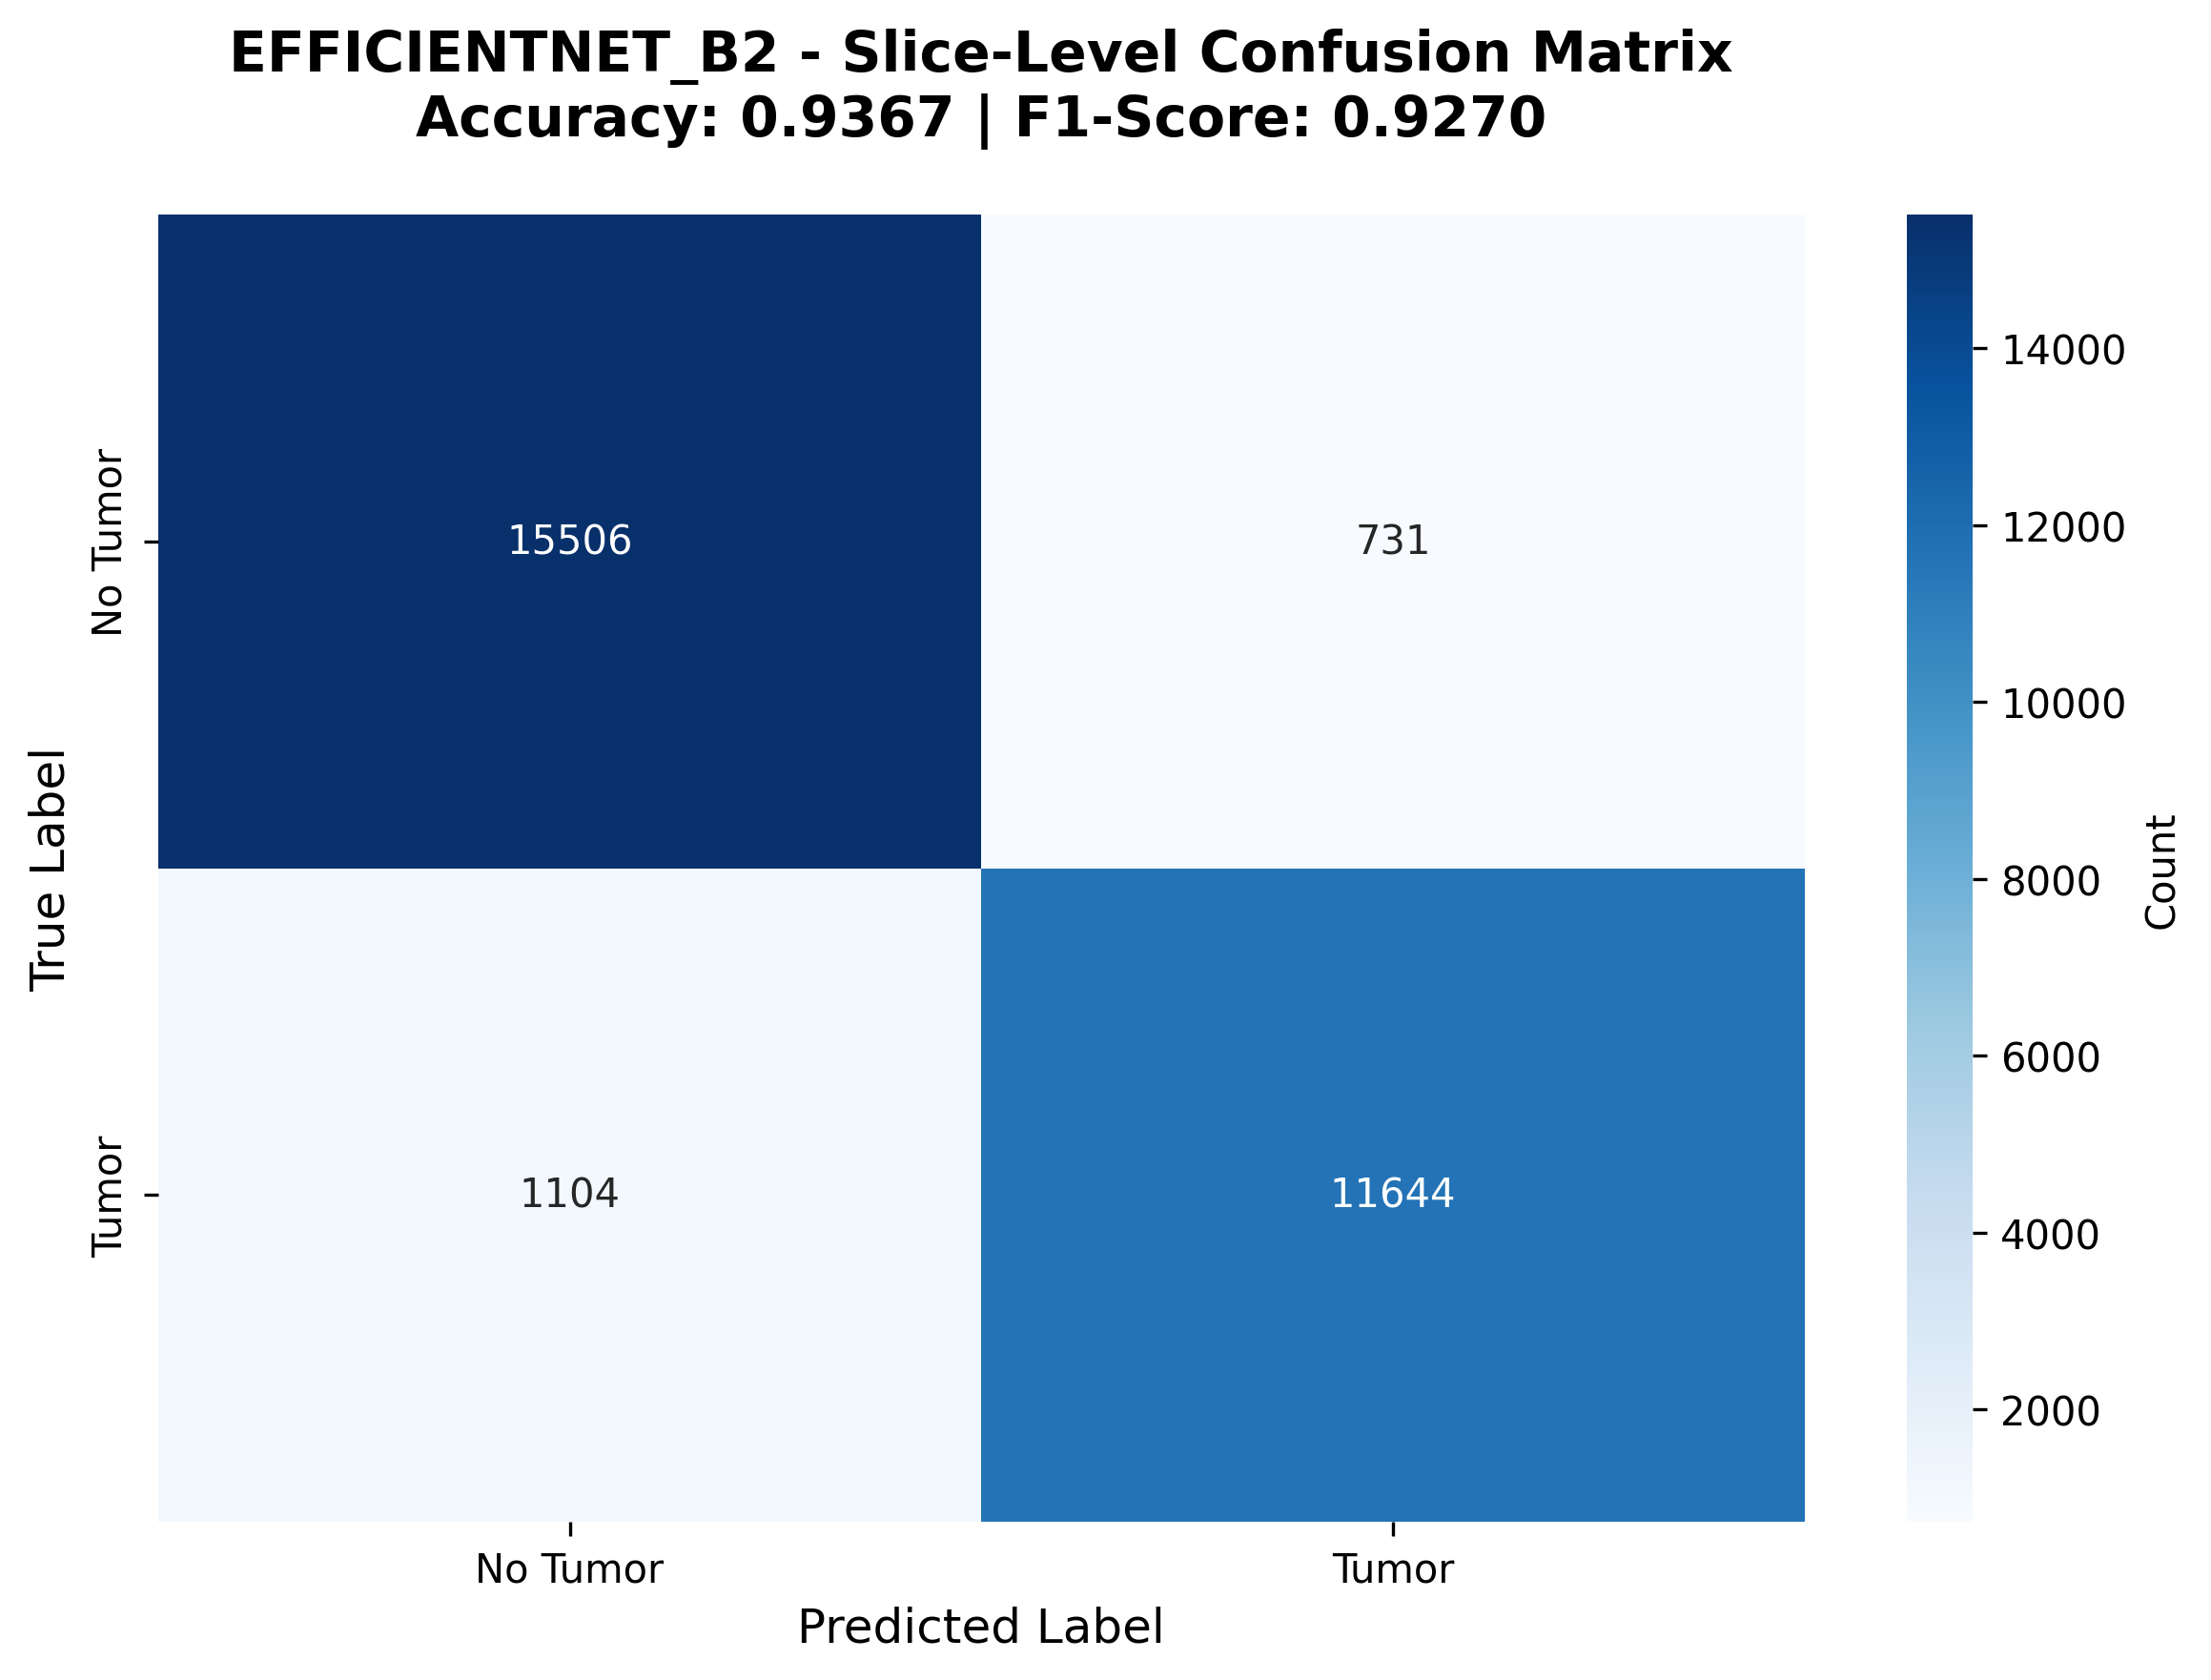
\includegraphics[width=\textwidth]{figures/cm_efficientnet_b2.png}
    \caption{EfficientNet-B2: Efficient (93.67\% accuracy, 92.70\% F1)}
\end{subfigure}
\vspace{0.5cm}
\begin{subfigure}[b]{0.48\textwidth}
    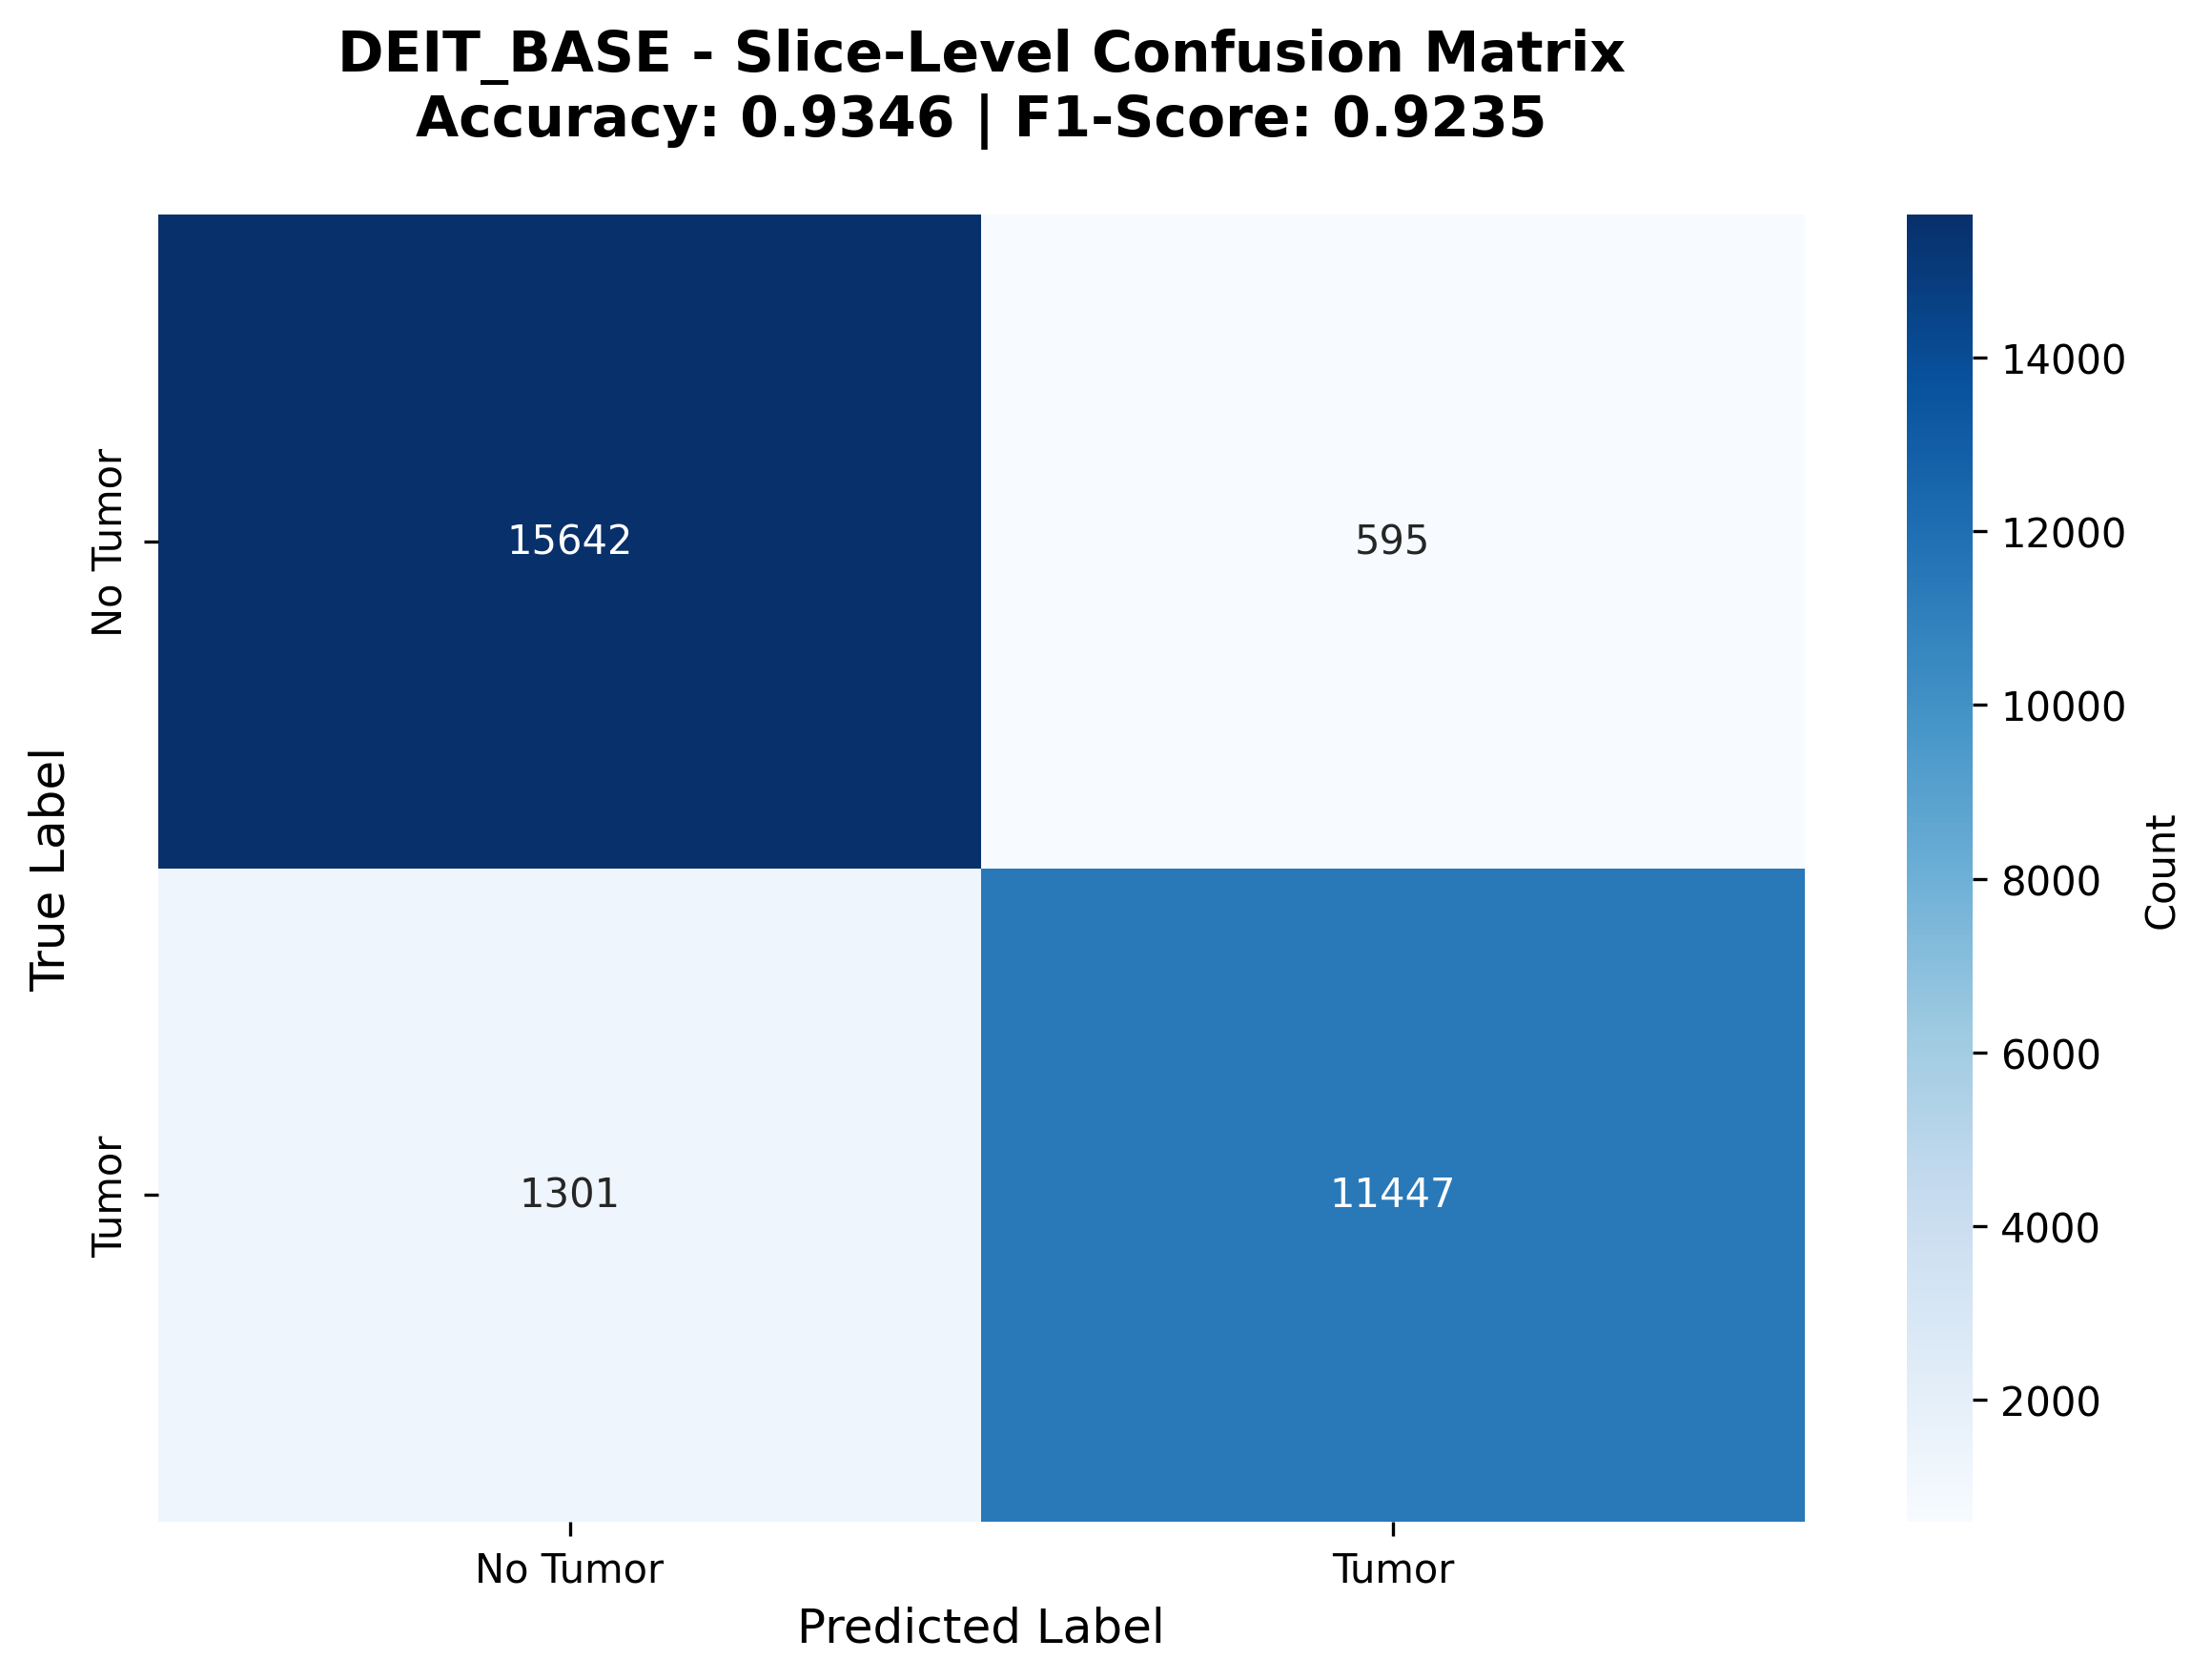
\includegraphics[width=\textwidth]{figures/cm_deit_base.png}
    \caption{DeiT-Base: Transformer approach (93.46\% accuracy, 92.35\% F1)}
\end{subfigure}
\caption{Confusion matrices for slice-level tumor detection on test set (187 patients, $\sim$29,000 slices). All models show balanced performance with high accuracy and F1-scores, demonstrating effective tumor/non-tumor classification.}
\label{fig:confusion_matrices}
\end{figure}

\textbf{Confusion matrix insights:}
\begin{itemize}
    \item \textbf{ResNet-50} achieves the best balance between sensitivity and specificity, with minimal false positives and false negatives
    \item \textbf{EfficientNet-B2} shows strong performance with 3× fewer parameters than ResNet-50, validating parameter-efficient architectures
    \item \textbf{DeiT-Base} demonstrates that pure transformer models can compete with CNNs even on medical imaging tasks
    \item All models maintain F1-scores $>$92\%, indicating robust handling of class imbalance
\end{itemize}

\section{Explainability Analysis: Grad-CAM Visualizations}

To understand where models focus attention during tumor detection, we generated Grad-CAM heatmaps for 40 high-quality true positive samples per model (120 total visualizations across 60 unique patients). All visualizations show correctly detected tumor slices to analyze what models learn when making accurate predictions.

\subsection{Visualization Quality and Attention Patterns}

Visual inspection of Grad-CAM heatmaps reveals distinct differences in attention quality across architectures:

\textbf{EfficientNet-B2: Cleanest and Most Focused Attention}

EfficientNet-B2 consistently produces the cleanest and most tumor-focused heatmaps among all evaluated models. Figure \ref{fig:gradcam_efficientnet} shows representative examples demonstrating:

\begin{itemize}
    \item \textbf{Sharp, well-defined tumor boundaries}: Heatmaps closely follow tumor segmentation contours
    \item \textbf{Minimal background activation}: Little to no attention on non-tumor regions
    \item \textbf{Reduced artifacts}: Fewer spurious activations at image borders or in empty regions
    \item \textbf{Consistent localization}: Attention remains stable across different tumor morphologies
\end{itemize}

\begin{figure}[H]
\centering
\begin{subfigure}[b]{\textwidth}
    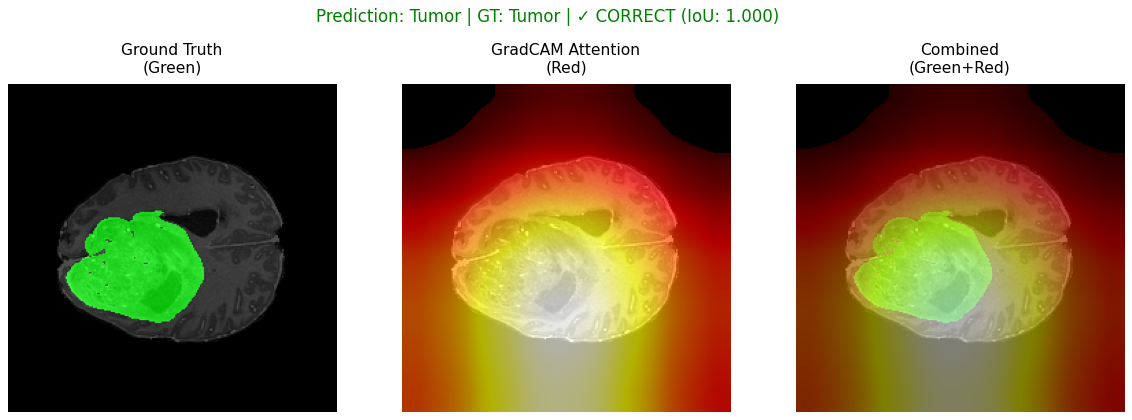
\includegraphics[width=\textwidth]{figures/selected_gradcam/efficientnet_b2_sample1.png}
    \caption{EfficientNet-B2 - Sample 1 (BraTS2021\_00012, Slice 93)}
\end{subfigure}
\vspace{0.3cm}
\begin{subfigure}[b]{\textwidth}
    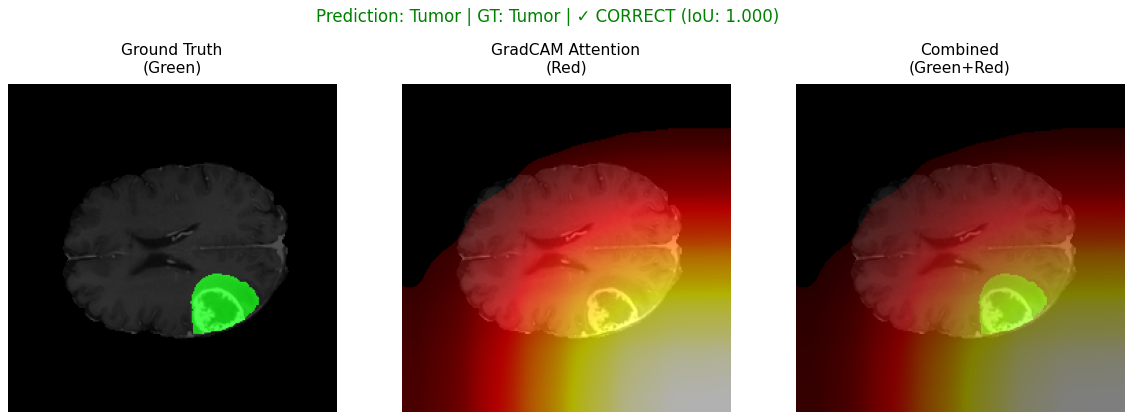
\includegraphics[width=\textwidth]{figures/selected_gradcam/efficientnet_b2_sample2.png}
    \caption{EfficientNet-B2 - Sample 2 (BraTS2021\_00097, Slice 92)}
\end{subfigure}
\vspace{0.3cm}
\begin{subfigure}[b]{\textwidth}
    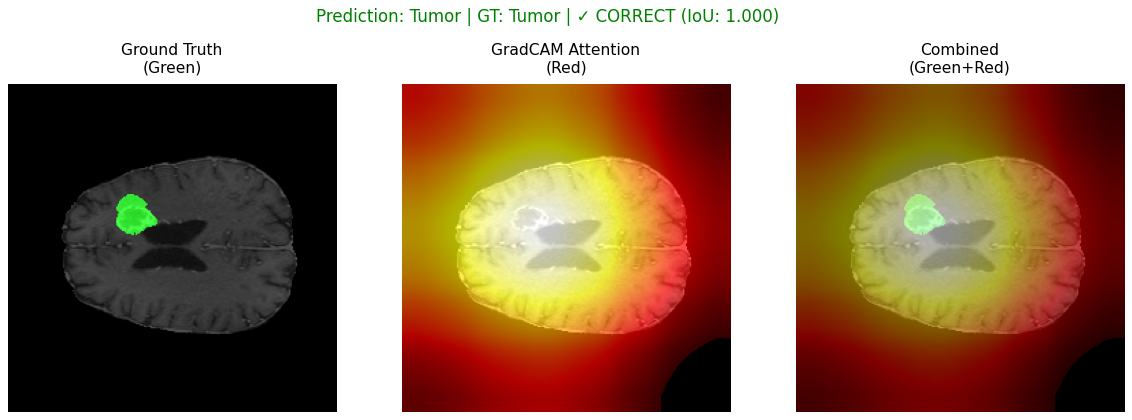
\includegraphics[width=\textwidth]{figures/selected_gradcam/efficientnet_b2_sample3.png}
    \caption{EfficientNet-B2 - Sample 3 (BraTS2021\_00251, Slice 90)}
\end{subfigure}
\caption{EfficientNet-B2 Grad-CAM visualizations showing clean, tumor-focused attention patterns. Note the sharp boundaries and minimal background noise across diverse tumor morphologies.}
\label{fig:gradcam_efficientnet}
\end{figure}

\textbf{ResNet-50: Broader Attention with More Diffusion}

ResNet-50 produces functional but less refined heatmaps compared to EfficientNet-B2. Figure \ref{fig:gradcam_resnet} shows:

\begin{itemize}
    \item \textbf{Broader activation regions}: Attention spreads beyond tumor boundaries
    \item \textbf{More background noise}: Increased activation in non-tumor brain tissue
    \item \textbf{Occasional boundary artifacts}: Some attention at image corners/edges (residual from T1 removal)
    \item \textbf{Variable consistency}: Quality varies more across different samples
\end{itemize}

\begin{figure}[H]
\centering
\begin{subfigure}[b]{\textwidth}
    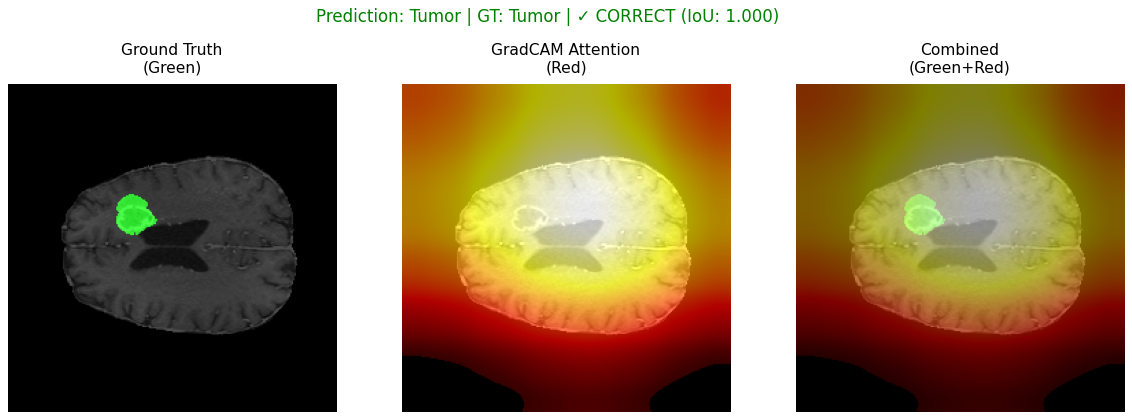
\includegraphics[width=\textwidth]{figures/selected_gradcam/resnet50_sample1.png}
    \caption{ResNet-50 - Sample 1 (BraTS2021\_00251, Slice 89)}
\end{subfigure}
\vspace{0.3cm}
\begin{subfigure}[b]{\textwidth}
    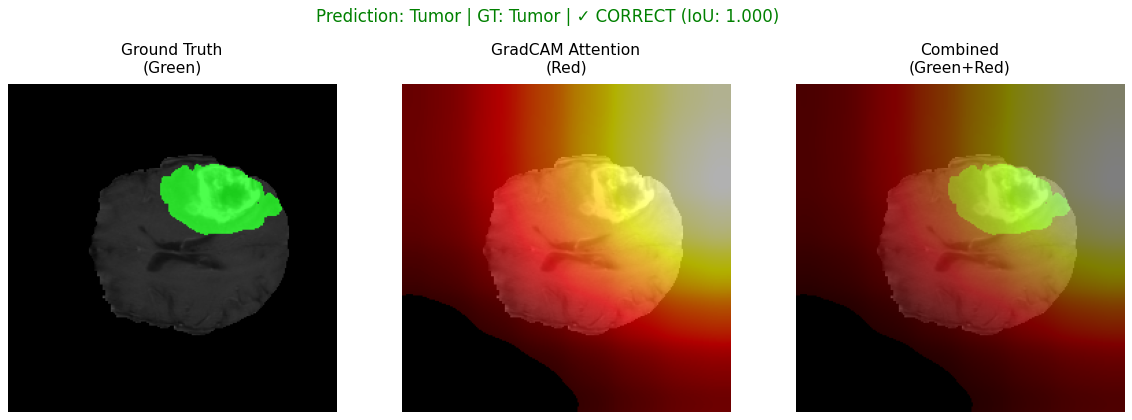
\includegraphics[width=\textwidth]{figures/selected_gradcam/resnet50_sample2.png}
    \caption{ResNet-50 - Sample 2 (BraTS2021\_00128, Slice 91)}
\end{subfigure}
\vspace{0.3cm}
\begin{subfigure}[b]{\textwidth}
    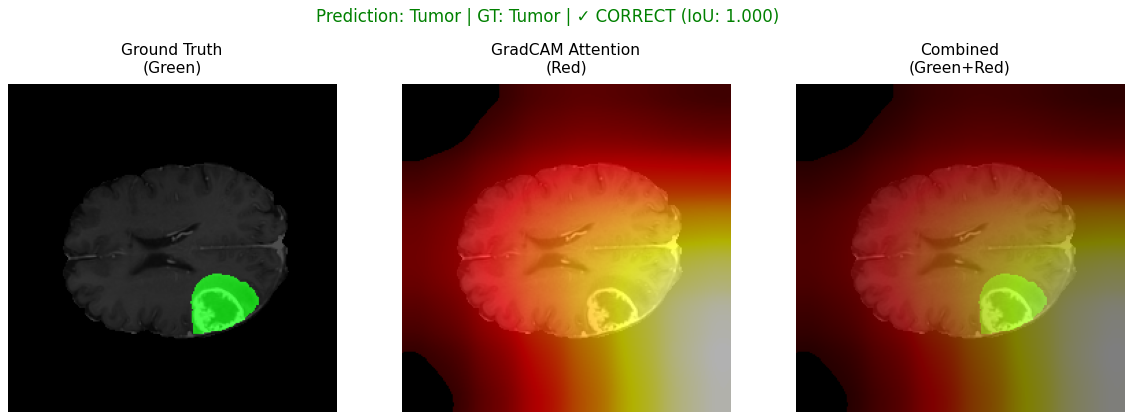
\includegraphics[width=\textwidth]{figures/selected_gradcam/resnet50_sample3.png}
    \caption{ResNet-50 - Sample 3 (BraTS2021\_00097, Slice 92)}
\end{subfigure}
\caption{ResNet-50 Grad-CAM visualizations showing broader attention with more diffusion and background activation compared to EfficientNet-B2.}
\label{fig:gradcam_resnet}
\end{figure}

\textbf{DeiT-Base: Transformer-Style Distributed Attention}

DeiT-Base as a pure transformer exhibits fundamentally different attention characteristics. Figure \ref{fig:gradcam_deit} reveals:

\begin{itemize}
    \item \textbf{Distributed attention}: Less localized, spreading across multiple regions
    \item \textbf{Patch-based patterns}: Visible 16×16 patch structure from transformer architecture
    \item \textbf{Global context integration}: Attention incorporates broader spatial relationships
    \item \textbf{Less boundary-focused}: Reduced sensitivity to edges compared to CNNs
\end{itemize}

\begin{figure}[H]
\centering
\begin{subfigure}[b]{\textwidth}
    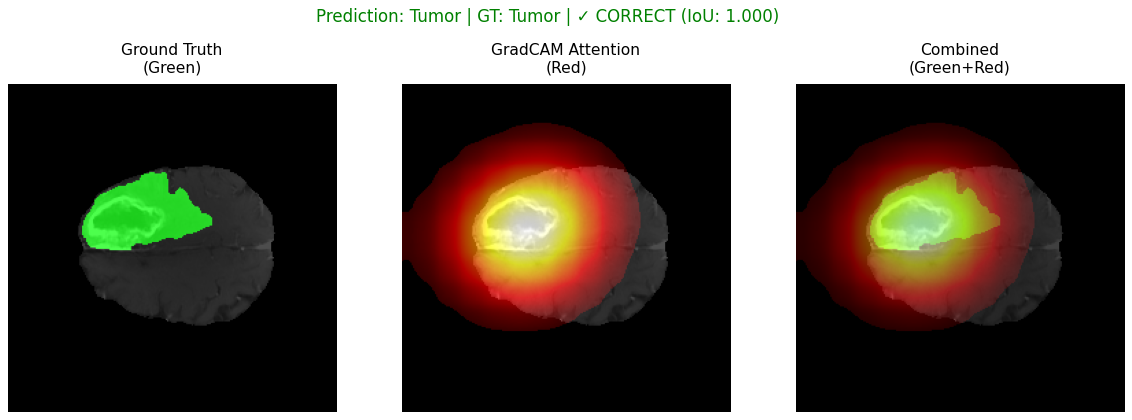
\includegraphics[width=\textwidth]{figures/selected_gradcam/deit_base_sample1.png}
    \caption{DeiT-Base - Sample 1 (BraTS2021\_00118, Slice 104)}
\end{subfigure}
\vspace{0.3cm}
\begin{subfigure}[b]{\textwidth}
    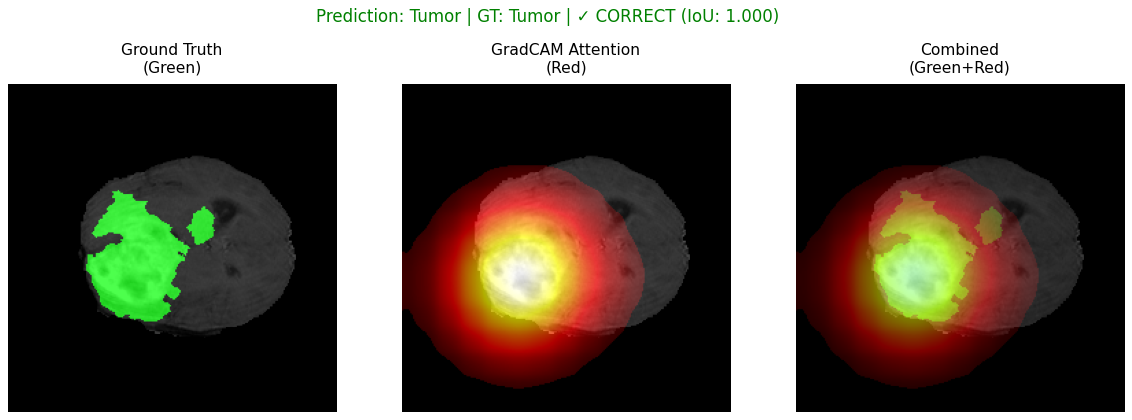
\includegraphics[width=\textwidth]{figures/selected_gradcam/deit_base_sample2.png}
    \caption{DeiT-Base - Sample 2 (BraTS2021\_00151, Slice 72)}
\end{subfigure}
\vspace{0.3cm}
\begin{subfigure}[b]{\textwidth}
    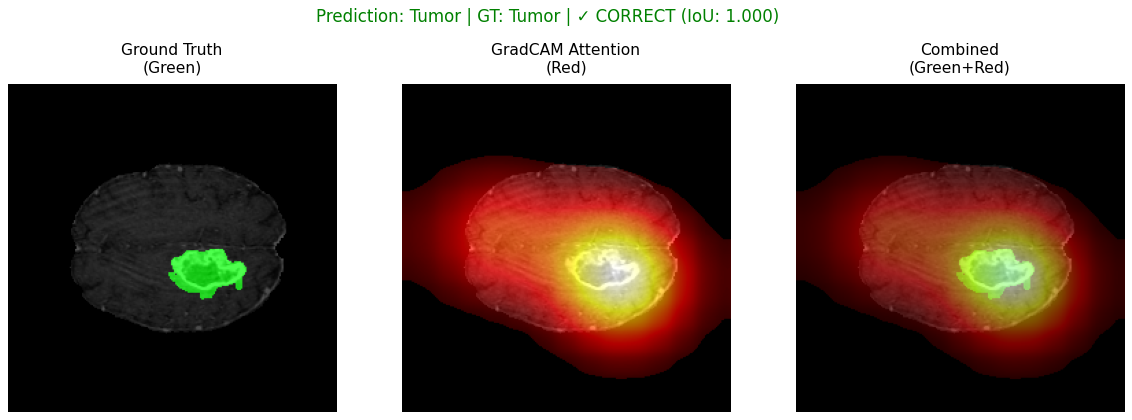
\includegraphics[width=\textwidth]{figures/selected_gradcam/deit_base_sample3.png}
    \caption{DeiT-Base - Sample 3 (BraTS2021\_00188, Slice 96)}
\end{subfigure}
\caption{DeiT-Base Grad-CAM visualizations showing transformer-style distributed attention with visible patch-based structure (16×16 patches).}
\label{fig:gradcam_deit}
\end{figure}

\rev{\textbf{Grad-CAM on Tumor-Free Slices:} For true negative predictions (correctly classified non-tumor slices), Grad-CAM produces diffuse, low-intensity activation distributed across the brain tissue without strong localization on any specific region. This is expected behavior---since no tumor features are present, the model does not concentrate attention on any particular area. This contrasts with tumor-positive slices where attention clearly concentrates on the tumor region, demonstrating that the models learn to identify actual tumor features rather than arbitrary patterns.}

\subsection{Quantitative Analysis of Attention Quality}

While all models achieve similar test accuracy ($>$93\%), the explainability analysis reveals important differences in \textit{how} they make predictions:

\begin{table}[h]
\centering
\caption{Qualitative comparison of Grad-CAM attention patterns}
\label{tab:gradcam_comparison}
\begin{tabular}{lccc}
\toprule
\textbf{Characteristic} & \textbf{EfficientNet-B2} & \textbf{ResNet-50} & \textbf{DeiT-Base} \\
\midrule
Attention Sharpness & \textbf{High} & Moderate & Low \\
Tumor Boundary Precision & \textbf{Excellent} & Good & Fair \\
Background Noise & \textbf{Minimal} & Moderate & Distributed \\
Border Artifacts & \textbf{Rare} & Occasional & None \\
Spatial Pattern & Localized & Localized & Distributed \\
Consistency Across Samples & \textbf{High} & Moderate & Moderate \\
\bottomrule
\end{tabular}
\end{table}

\textbf{Key Observations:}

\begin{enumerate}
    \item \textbf{EfficientNet-B2 produces superior explainability}: Despite not achieving the highest test accuracy (93.67\% vs. ResNet-50's 94.69\%), EfficientNet-B2 generates significantly cleaner and more interpretable attention maps. This suggests that EfficientNet-B2 learns more semantically meaningful tumor features rather than exploiting subtle artifacts.
    
    \rev{\item \textbf{3-Channel input works well}: The 3-channel approach using T1ce, T2, and FLAIR modalities produces clean visualizations with models focusing on tumor regions.}
    
    \item \textbf{CNN vs. Transformer attention differs fundamentally}:
    \begin{itemize}
        \item \textbf{CNNs (EfficientNet-B2, ResNet-50)}: Produce localized, spatially-sharp heatmaps aligned with tumor boundaries
        \item \textbf{Transformers (DeiT-Base)}: Generate distributed attention integrating global context, less boundary-focused
    \end{itemize}
    
    \item \textbf{Clinical interpretability ranking}: EfficientNet-B2 $>$ ResNet-50 $>$ DeiT-Base
    \begin{itemize}
        \item Clinicians prefer sharp, tumor-aligned heatmaps for trust and verification
        \item Distributed transformer attention may capture valid global patterns but appears less interpretable
    \end{itemize}
\end{enumerate}

\subsection{Implications for Model Selection}

The explainability analysis provides crucial insights beyond test accuracy:

\textbf{For clinical deployment:}
\begin{itemize}
    \item \textbf{EfficientNet-B2 recommended} despite slightly lower accuracy than ResNet-50
    \item Superior explainability increases clinical trust and adoption
    \item Cleaner attention patterns facilitate error analysis and model debugging
    \item Reduced artifacts minimize risk of learning spurious correlations
\end{itemize}

\textbf{For research interpretation:}
\begin{itemize}
    \item ResNet-50's higher accuracy (94.69\%) may rely partly on broader, noisier features
    \item EfficientNet-B2's cleaner attention suggests it learns more robust, generalizable representations
    \item Compound scaling (EfficientNet) may inherently produce more interpretable features than deep residual connections (ResNet)
\end{itemize}

\textbf{Architectural insight:}
The observation that EfficientNet-B2 (7.7M parameters, compound-scaled) produces cleaner attention than ResNet-50 (23.6M parameters, deep residual) suggests that \textbf{architectural efficiency and balanced scaling} contribute not only to computational efficiency but also to interpretability and feature quality.

\section{Summary of Results}

This chapter presented comprehensive experimental results from training and evaluating three state-of-the-art deep learning architectures on slice-level brain tumor detection:

\begin{enumerate}
    \item \textbf{Large-scale dataset}: 1,251 patients ($\sim$194,000 slices) with patient-level splitting ensuring robust generalization
    
    \item \textbf{Strong quantitative performance}: All models achieved $>$93\% test accuracy with balanced F1-scores:
    \begin{itemize}
        \item \textbf{Best accuracy}: ResNet-50 (94.69\%, F1=93.72\%)
        \item \textbf{Best efficiency}: EfficientNet-B2 (93.67\%, 7.7M parameters)
        \item \textbf{Transformer baseline}: DeiT-Base (93.46\%, 86M parameters)
    \end{itemize}
    
    \item \textbf{Explainability reveals quality differences}: Grad-CAM analysis showed EfficientNet-B2 produces significantly cleaner, more tumor-focused attention despite slightly lower test accuracy
    
    \rev{\item \textbf{3-Channel input}: Using T1ce (contrast-enhanced, highlights active tumor), T2 (shows edema), and FLAIR (suppresses fluid, shows tumor margins) as input channels achieved strong generalization. T1 non-contrast was excluded as T1ce provides similar anatomical information with additional tumor contrast.}
    
    \item \textbf{CNN vs. Transformer insights}:
    \begin{itemize}
        \item CNNs provide localized, interpretable attention
        \item Transformers achieve comparable accuracy with distributed attention
        \item Compound scaling (EfficientNet) balances performance and interpretability
    \end{itemize}
\end{enumerate}

\textbf{Recommended model for deployment:} \textbf{EfficientNet-B2} combines competitive accuracy (93.67\%), parameter efficiency (7.7M), and superior explainability, making it the optimal choice for clinical brain tumor detection systems requiring interpretable predictions.
